\documentclass[11pt, a4paper]{article}

% ── Lengua ─────────────────────────────
\usepackage[utf8]{inputenc}
\usepackage[T1]{fontenc}
\usepackage[spanish]{babel}

% ── Fuentes compatibles pdflatex ───────
\usepackage{lmodern}
\usepackage{courier}

% ── Interlineado ───────────────────────
\usepackage{setspace}
\onehalfspacing

% ── Márgenes ───────────────────────────
\usepackage[a4paper, margin=2.5cm]{geometry}

% ── Cabecera/pie ───────────────────────
\usepackage{fancyhdr}
\pagestyle{fancy}
\fancyhf{}
\rfoot{\thepage}
\renewcommand{\headrulewidth}{0pt}

% ── Imágenes ───────────────────────────
\usepackage{graphicx}
\graphicspath{{imgs/}}
\usepackage{subcaption}

% ── Links ──────────────────────────────
\usepackage[hidelinks]{hyperref}

% ── Código ─────────────────────────────
\usepackage{listings}
\lstset{
  basicstyle=\ttfamily\footnotesize,
  breaklines=true,
  frame=single,
  numbers=left,
  numberstyle=\tiny
}

% ── Documento ───────────────────────────
\begin{document}

% ── PORTADA ─────────────────────────────
\begin{titlepage}
\centering

% empuja todo hacia el centro vertical
\vspace*{\fill}

{\Huge \textbf{Actividad2: Laboratorio Uso de MongoDB}\par}

\vspace{1.5cm}

{\Large David Vicente Moya\par}

\vspace{0.5cm}

{\large \today\par}

% relleno inferior para centrar verticalmente
\vspace*{\fill}

\end{titlepage}

% ── ÍNDICE ──────────────────────────────
\newpage
\tableofcontents
\thispagestyle{empty}
\setcounter{page}{0}

% ── CONTENIDO ──────────────────────────
\newpage

% Apartado 1
\section{Carga de fichero y esquema de datos}

Para cargar los datos en MongoDB primero he creado un nuevo contenedor específico para 
esta actividad, en un puerto libre:

\begin{lstlisting}[language=bash]
docker run --name Actividad2DBDB -d -p 27019:27017 mongo
\end{lstlisting}

Seguido de esto, con Mongo Compass he creado una nueva base de datos llamada ``Proyecto'' 
y he importado los ficheros JSON en las colecciones ``books'' y ``companies''. Para la 
carga de datos se han usado los siguientes comandos (he acortado la dirección de los
ficheros en este extracto):

\begin{lstlisting}[language=bash]
mongoimport --verbose --port 27019 --db Proyecto --collection books --file C:\...\act-2-books.json
mongoimport --verbose --port 27019 --db Proyecto --collection companies --file C:\...\act-2-companies.json
\end{lstlisting}

\section{Exploración de las colecciones}
\subsection*{a)}
\begin{lstlisting}
// Obtengo una muestra de cada coleccion para ver su estructura.
db.books.findOne()
db.companies.findOne()
\end{lstlisting}

\begin{figure}[h]
    \centering

    \begin{subfigure}{0.49\textwidth}
        \centering
        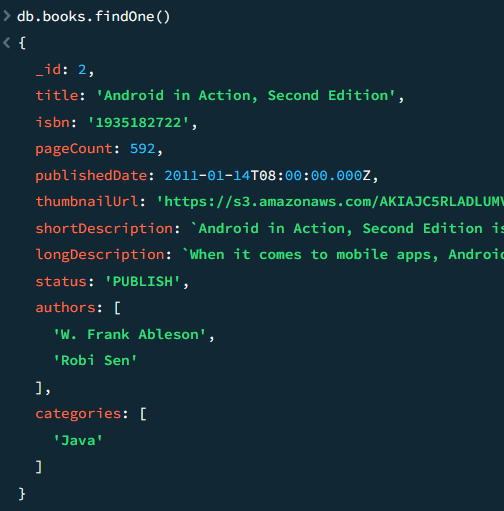
\includegraphics[width=\linewidth]{find_books.png}
        \caption{Colección books.}
        \label{fig:find-books}
    \end{subfigure}
    \hfill
    \begin{subfigure}{0.49\textwidth}
        \centering
        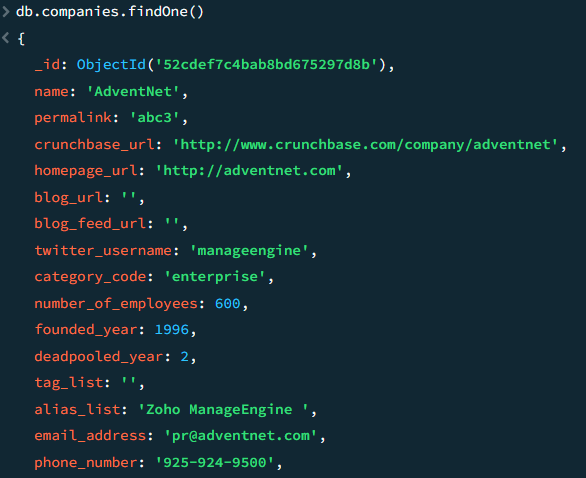
\includegraphics[width=\linewidth]{find_companies.png}
        \caption{Colección companies.}
        \label{fig:find-companies}
    \end{subfigure}

    \caption{Búsqueda del primer documento de cada colección.}
    \label{fig:find-collections}
\end{figure}

Los resultados de estas consultas no han sido incluidos en el informe para evitar que 
la extensión del mismo sobrepase las 10 páginas, tal y como se especifica en el 
enunciado. Gracias a estas consultas he podido identificar  dos campos categóricos de 
cada collección:

\begin{itemize}
    \item En la colección \textbf{books}:
    \begin{itemize}
        \item \texttt{status}: estado de publicación del libro.
        \item \texttt{categories}: categorías a las que pertenece el libro.
    \end{itemize}
    \item En la colección \textbf{companies}:
    \begin{itemize}
        \item \texttt{category\_code}: la categoría a la que pertenece la empresa.
        \item \texttt{offices.country\_code}: el país en el que se encuentran las oficinas.
    \end{itemize}
\end{itemize}

\begin{lstlisting}
// Busco todos los valores unicos para las variables categoricas de books.
db.books.distinct("status")
db.books.distinct("categories")

// Busco todos los valores unicos para las variables categoricas de companies.
db.companies.distinct("category_code")
db.companies.distinct("offices.country_code")
\end{lstlisting}
\begin{figure}[h]
    \centering

    \begin{subfigure}{0.4\textwidth}
        \centering
        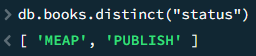
\includegraphics[width=\linewidth]{distinct_status.png}
        \caption{Estados posibles de un libro.}
        \label{fig:distinct-status}
    \end{subfigure}
    \hfill
    \begin{subfigure}{0.4\textwidth}
        \centering
        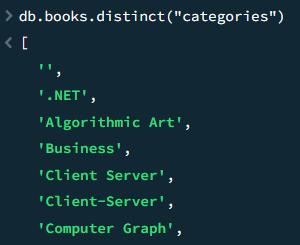
\includegraphics[width=\linewidth]{distinct_categories.png}
        \caption{Categorías de los libros.}
        \label{fig:distinct-categories}
    \end{subfigure}

    \caption{Resultados de realizar distinct sobre variables categóricas de la colección books.}
    \label{fig:distinct-books}
\end{figure}

\begin{figure}[h]
    \centering

    \begin{subfigure}{0.43\textwidth}
        \centering
        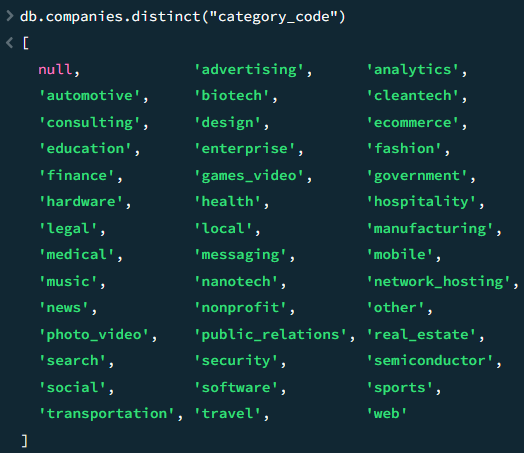
\includegraphics[width=\linewidth]{distinct_category_code.png}
        \caption{Códigos de categoría de las empresas.}
        \label{fig:distinct-category-code}
    \end{subfigure}
    \hfill
    \begin{subfigure}{0.43\textwidth}
        \centering
        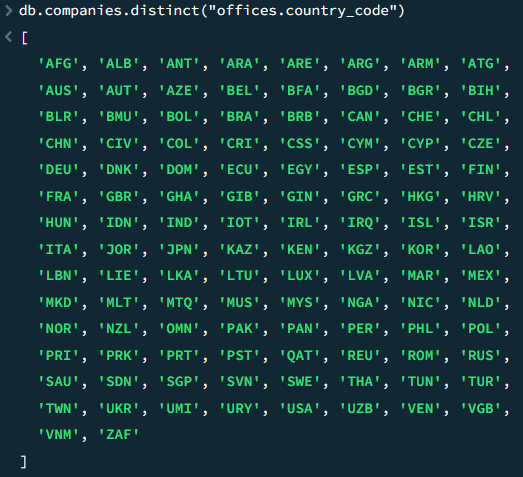
\includegraphics[width=\linewidth]{distinct_country_code.png}
        \caption{Códigos de país de las oficinas.}
        \label{fig:distinct-country-code}
    \end{subfigure}

    \caption{Resultados de realizar distinct sobre variables categóricas de la colección companies.}
    \label{fig:distinct-companies}
\end{figure}

\subsection*{b)}

\begin{lstlisting}
db.getCollection('companies').find(
    { number_of_employees: {$gte: 500, $lt: 1000}}, 
    { name: 1, homepage_url: 1 }
)
\end{lstlisting}

\begin{figure}[h]
    \centering
    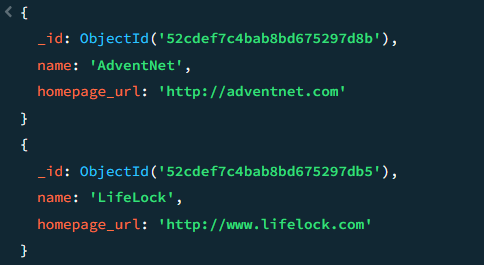
\includegraphics[width=0.5\textwidth]{apartado2b.png}
    \caption{Apartado 2b: empresas con entre 500 y 1000 empleados.}
    \label{fig:apartado2b}
\end{figure}

\subsection*{c)}

\begin{lstlisting}
db.getCollection('companies').find(
  {
    number_of_employees: {$gte: 500, $lt: 1000},
    phone_number: { $exists: true },
    homepage_url: { $type: "string" }
  },
  { _id: 0, name: 1, number_of_employees: 1, homepage_url: 1, phone_number: 1 }
)
\end{lstlisting}

\begin{figure}[h]
    \centering
    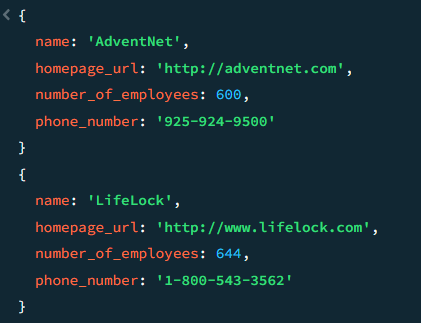
\includegraphics[width=0.55\textwidth]{apartado2c.png}
    \caption{Apartado 2c: empresas con entre 500 y 1000 empleados y datos completos.}
    \label{fig:apartado2c}
\end{figure}

\subsection*{d)}

Al utilizar \texttt{.toArray()} al final de la consulta, el resultado se devuelve como 
un array de documentos.

\subsection*{e)}
\begin{lstlisting}
db.getCollection('companies').find(
  {
    number_of_employees: {$gte: 500, $lt: 1000},
    phone_number: { $exists: true },
    homepage_url: { $type: "string" }
  },
  { _id: 0, name: 1, number_of_employees: 1, homepage_url: 1, phone_number: 1 }
).forEach(function(valor, indice, array) {
  print(
    "Empresa: " + valor.name +
    " | Empleados: " + valor.number_of_employees +
    " | Web: " + valor.homepage_url +
    " | Telefono: " + valor.phone_number +
    " | Registro No. " + indice
  )
})
\end{lstlisting}

\begin{figure}[h]
    \centering
    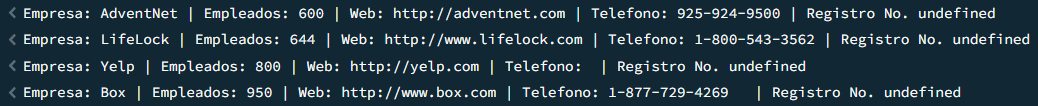
\includegraphics[width=0.99\textwidth]{apartado2e.png}
    \caption{Apartado 2e: empresas con entre 500 y 1000 empleados y datos completos mostrados de informe.}
    \label{fig:apartado2e}
\end{figure}

Imprime en consola una línea formateada, por cada documento que cumple las condiciones, 
que contiene los datos buscados. Se podría utilizar para generar informes dinámicos 
desde consola sin necesidad de usar herramientas externas.

\section{Consultas en la colección \texttt{books}}

\subsection*{a)}
\begin{lstlisting}
// Tamano de la coleccion books en bytes.
db.books.dataSize()
> 517474 B
\end{lstlisting}

\subsection*{b)}
\begin{lstlisting}
// Numero de documentos de la coleccion books.
db.books.countDocuments()
> 431
\end{lstlisting}

\subsection*{c)}
\begin{lstlisting}
// Libros con mas de 300 paginas y menos de 600
db.books.find(
  { pageCount: { $gt: 300, $lt: 600 } },
  { _id: 0, title: 1, pageCount: 1 }
)
\end{lstlisting}

\begin{figure}[h]
    \centering
    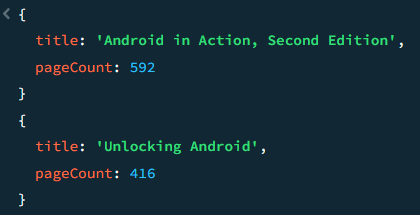
\includegraphics[width=0.6\textwidth]{apartado3c.png}
    \caption{Apartado 3c: libros con entre 300 y 600 páginas.}
    \label{fig:apartado3c}
\end{figure}

\subsection*{d)}
\begin{lstlisting}
// Libros con entre 400 y 700 paginas y estado PUBLISH
db.books.find(
  {
    $and: [
      { pageCount: { $gte: 400 } },
      { pageCount: { $lte: 700 } },
      { status: "PUBLISH" }
    ]
  },
  { _id: 0, title: 1, pageCount: 1, status: 1 }
)
\end{lstlisting}

\begin{figure}[h]
    \centering
    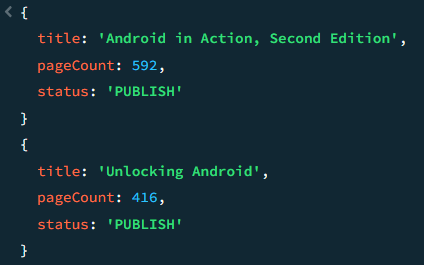
\includegraphics[width=0.6\textwidth]{apartado3d.png}
    \caption{Apartado 3d: libros con entre 400 y 700 páginas y estado PUBLISH.}
    \label{fig:apartado3d}
\end{figure}

\subsection*{e)}
\begin{lstlisting}
// Estadisticas de paginas de libros con pageCount mayor que 0.
db.books.aggregate([
  { $match: { pageCount: { $gt: 0 } } },
  {
    $group: {
      _id: null,
      max_paginas: { $max: "$pageCount" },
      min_paginas: { $min: "$pageCount" },
      media_paginas: { $avg: "$pageCount" }
    }
  }
])
\end{lstlisting}

\begin{figure}[h]
    \centering
    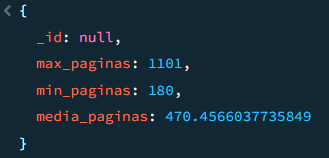
\includegraphics[width=0.45\textwidth]{apartado3e.png}
    \caption{Apartado 3e: estadísticas de páginas de libros con pageCount mayor que 0.}
    \label{fig:apartado3e}
\end{figure}

\subsection*{f)}
\begin{lstlisting}
// Total de documentos agrupados por status.
db.books.aggregate([
  {
    $group: {
      _id: "$status",
      total: { $sum: 1 }
    }
  },
  { $sort: { total: -1 } }
])
\end{lstlisting}

\begin{figure}[h]
    \centering
    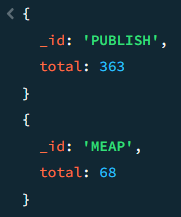
\includegraphics[width=0.23\textwidth]{apartado3f.png}
    \caption{Apartado 3f: distribución de libros por estado.}
    \label{fig:apartado3f}
\end{figure}

\section{Consultas en la colección \texttt{companies}}

\subsection*{a)}
\begin{lstlisting}
// Tamano de la coleccion companies en bytes.
db.companies.dataSize()
> 72236994 B
\end{lstlisting}

\subsection*{b)}
\begin{lstlisting}
// Numero de documentos de la coleccion companies.
db.companies.countDocuments()
> 18801
\end{lstlisting}

\subsection*{c)}
\begin{lstlisting}
// Empresas que pertenecen a alguna de estas categorias
db.companies.find(
  { category_code: { $in: ["software", "web", "mobile", "games_video"] } },
  { _id: 0, name: 1, category_code: 1 }
)
\end{lstlisting}

\begin{figure}[h]
    \centering
    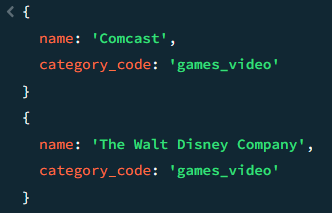
\includegraphics[width=0.5\textwidth]{apartado4c.png}
    \caption{Apartado 4c: empresas en categorías específicas.}
    \label{fig:apartado4c}
\end{figure}

\subsection*{d)}
\begin{lstlisting}
db.companies.aggregate([
  {
    $project: {
      _id: 0,
      name: 1,
      category_code: 1,
      homepage_url: 1
    }
  },
  {
    $match: {
      name: { $type: "string" },
      category_code: { $type: "string" },
      homepage_url: { $type: "string" }    }
  },
  {
    $out: "companies_report"
  }
])
\end{lstlisting}
\begin{figure}[h]
    \centering
    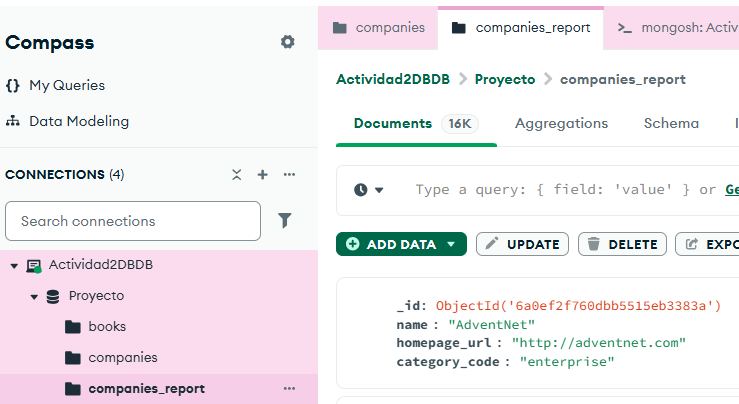
\includegraphics[width=0.8\textwidth]{companies_report.png}
    \caption{Output de agregación con \texttt{\$out} de un informe sobre companies.}
    \label{fig:companies-report}
\end{figure}

\subsection*{e)}
\begin{lstlisting}
// $match
// Companias de software con mas de 100 empleados
{
  category_code: { $in: ['software', 'web', 'mobile'] },
  number_of_employees: { $gte: 100 }
}

// $unwind
// Separo los productos de cada documento
{
  path: '$products',
  preserveNullAndEmptyArrays: false
}

// $project
// Me quedo con los datos que mas me interesan
{
  _id: 0,
  name: 1,
  homepage_url: 1,
  category_code: 1,
  number_of_employees: 1,
  founded_year: 1,
  product: '$products'
}

// $sort
// Ordeno segun el numero de empleados de forma descendiente
{
  number_of_employees: -1
}

// $out
// Guardo el resultado en una nueva coleccion a modo de informe
{
  db: 'Proyecto',
  coll: 'great_software_products_report',
}
\end{lstlisting}

\begin{figure}[h]
    \centering
    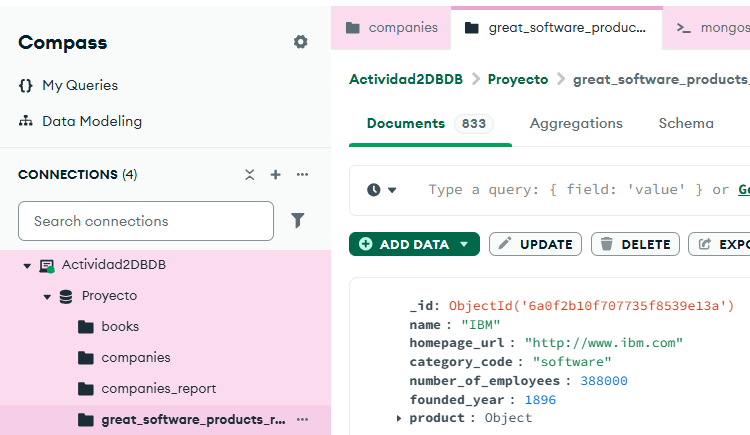
\includegraphics[width=0.8\textwidth]{great_software_products_report.png}
    \caption{Output de pipeline deagregación sobre companies.}
    \label{fig:great-software-products-report}
\end{figure}

\subsection*{f)}
\begin{lstlisting}
// Indice compuesto
db.companies.createIndex(
  { category_code: 1, number_of_employees: -1 },
  { name: "idx_categoria_empleados" }
)

// Indice simple 1
db.companies.createIndex(
  { name: 1 },
  { name: "idx_nombre" }
)

// Indice simple 2
db.companies.createIndex(
  { founded_year: 1 },
  { name: "idx_ano_fundacion" }
)

// Indice simple 3
db.companies.createIndex(
  { founded_month: 1 },
  { name: "idx_mes_fundacion" }
)

// Indice de texto
db.companies.createIndex(
  { description: "text", overview: "text" },
  { name: "idx_texto_descripcion" }
)
\end{lstlisting}

\begin{figure}[h]
    \centering
    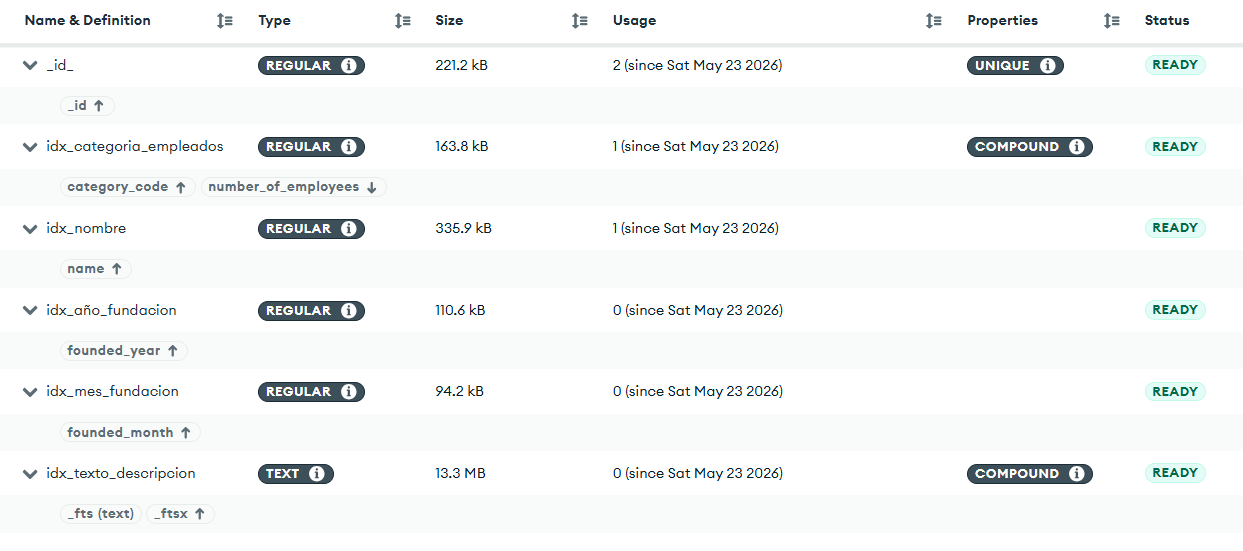
\includegraphics[width=0.99\textwidth]{indices.png}
    \caption{Indices creados en la colección companies.}
    \label{fig:indices}
\end{figure}

\subsection*{g)}

\begin{lstlisting}
// Buscar empresas cuya descripcion contenga "social network"
db.companies.find(
  { $text: { $search: "social network" } },
  { 
    _id: 0,
    name: 1,
    description: 1,
    score: { $meta: "textScore" }
  }
).sort({ score: { $meta: "textScore" } })
\end{lstlisting}

\begin{figure}[h]
    \centering
    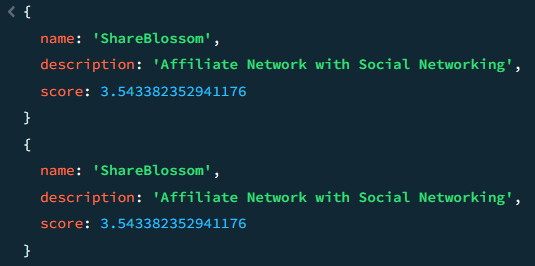
\includegraphics[width=0.8\textwidth]{apartado4g.png}
    \caption{Apartado 4g: empresas con ``social network'' en la descripción.}
    \label{fig:apartado4g}
\end{figure}

\end{document}